\section{Dynamic stem under calibrated forces}
\label{sec:supp-dynamic-stem}

\paragraph{A scale ambiguity with an external test.}
The stem has a $0.08\times0.08$ m square cross-section and free length $L=0.40$ m. A clamp fixes the first 0.04 m of its 0.44 m total length. The three material settings pair densities $\rho=500,1000,2000$ kg/m$^3$ with Young's moduli $E=2,4,8$ MPa, respectively. All have Poisson ratio 0.3. For motion driven by gravity from the same undeformed, stationary initial state, mass, gravitational loading and elastic restoring forces scale together. Dividing the equations of motion by $\rho$ leaves the common ratio $E/\rho$. The nonlinear reference simulations agree to within $4\times10^{-17}$ m during passive release. A prescribed force in newtons breaks this symmetry.

At 48 frames/s we observe a passive release (D0, 0.5 s) and optionally a second release with a 40 N lateral load distributed around $0.50L$ (D1, 0.75 s). The force rises with a 0.25 s cosine ramp. D2 applies 20 N laterally at $0.75L$. The fresh diagonal test D2b applies 15 N downward and 20 N laterally at the same station. For the D2 lateral target, an estimator that predicts one peak for both extreme worlds must miss at least one peak by $(30.7-7.7)/2=11.5$ mm to the reported precision. This bound concerns peak displacement at $0.75L$. We score displacement trajectories separately.

\paragraph{Reference and visual baseline.}
The reference integrates compressible Neo-Hookean dynamics using quadratic tetrahedra on a $33\times6\times6$ cell grid, implicit Newmark time integration and Newton iteration. On the largest calibration response, a coarser mesh changed station displacement by 0.16 mm RMS and halving the time step changed it by 0.07 mm, compared with 25.7 mm of motion. Our lower-resolution linear-elastic model uses the same element family. GIC reconstructs its particles from RGB. Its material-point simulator fits one global $E$, Poisson ratio and initial velocity with density fixed at 1000 kg/m$^3$. The calibrated-force adapter adds the specified momentum to its grid and propagates its derivative. A zero-force replay agreed with native simulation within GPU run-to-run variability, while a momentum check gave a 0.18\% difference. GIC refits on the calibration episode from its initial estimate, whereas our posterior multiplies the likelihoods of the two episodes.

\begin{figure*}[t]
\centering
\IfFileExists{figures/fig4-predicted-shapes.pdf}{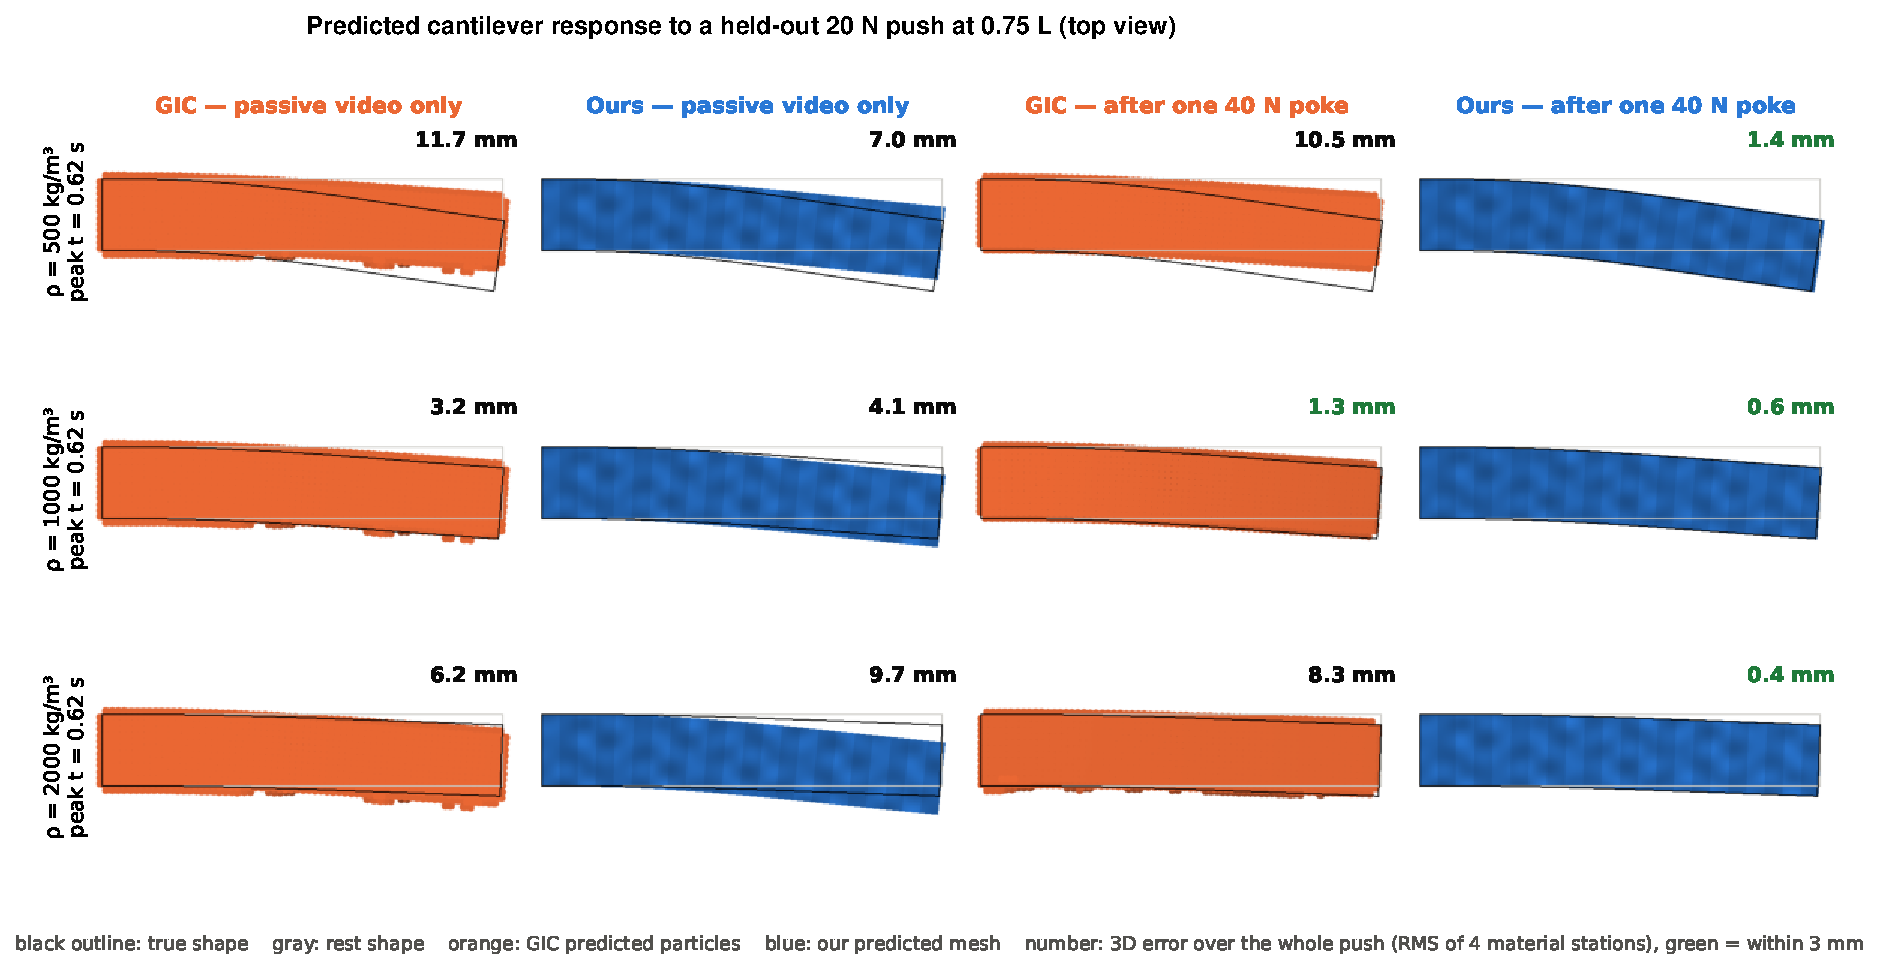
\includegraphics[width=.97\textwidth]{figures/fig4-predicted-shapes.pdf}}{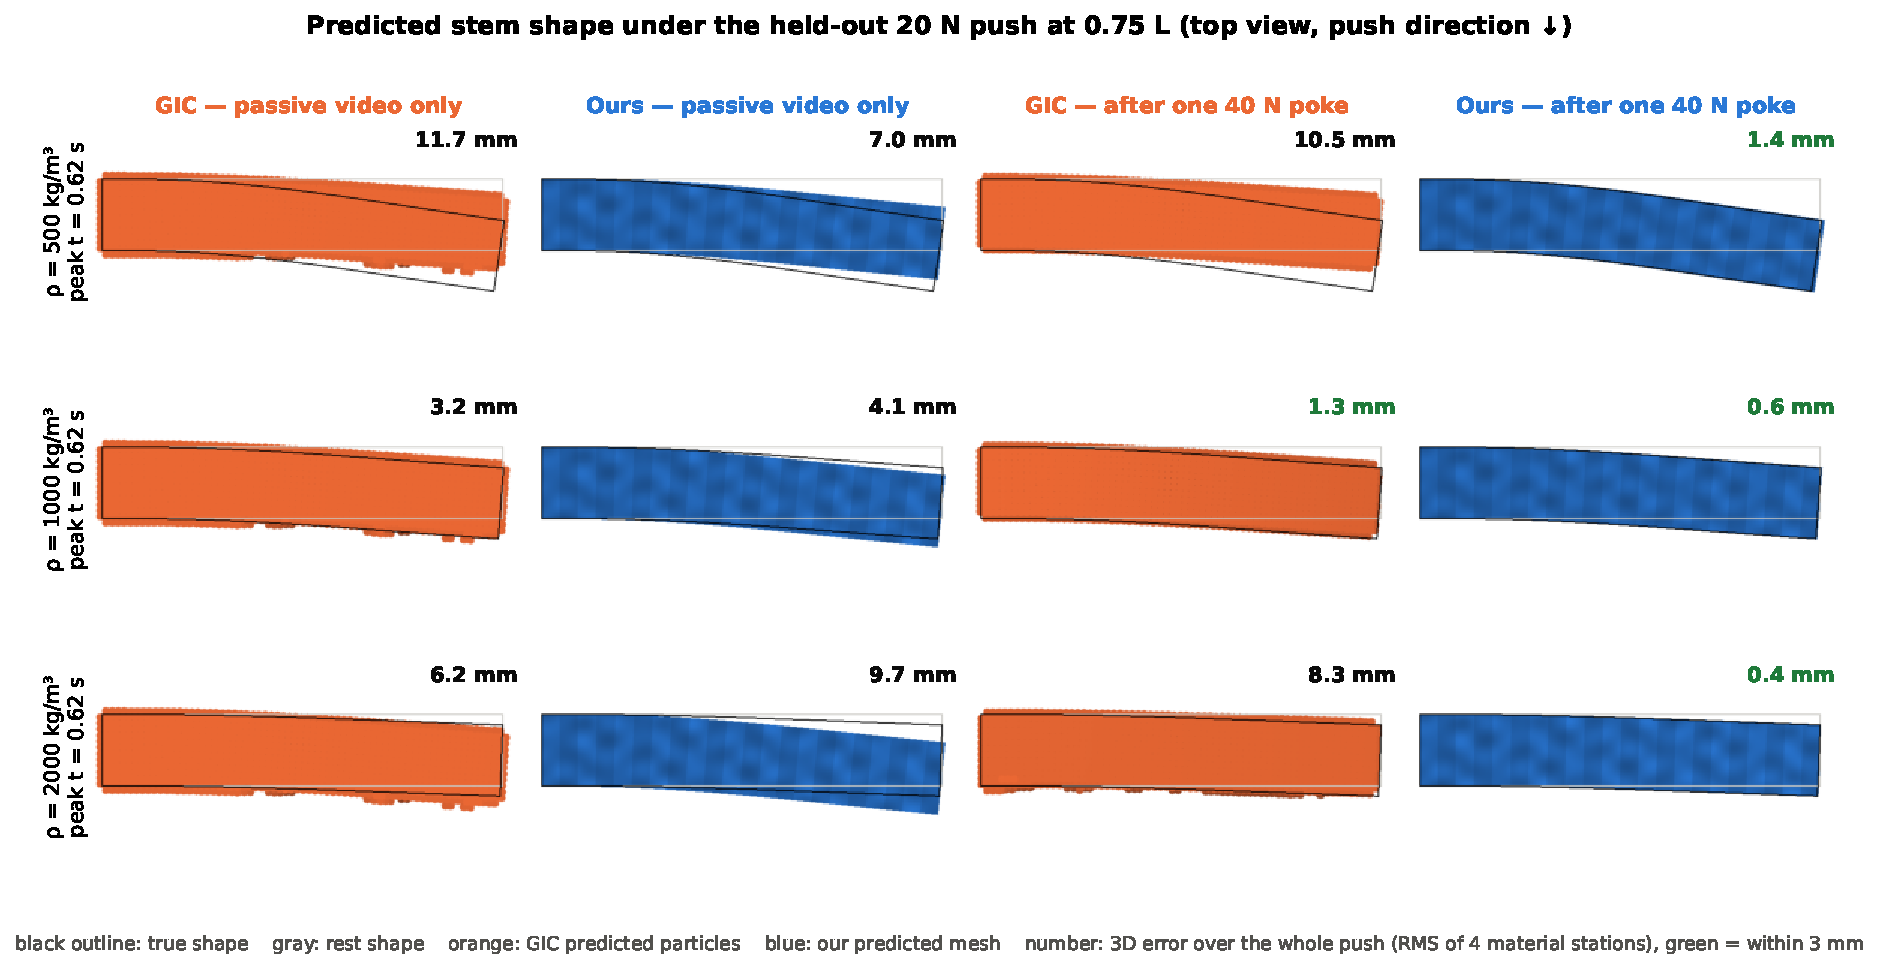
\includegraphics[width=.97\textwidth]{../../output/paper-figures/fig4-predicted-shapes.pdf}}
\caption{Top views at each reference stem's peak lateral tip displacement under the 20 N test push (D2). Gray and black outlines denote the rest shape and the nonlinear reference, respectively. Orange shows the GIC particle reconstruction from RGB. Blue shows the posterior-mean FEM field inferred from eight supplied 3D tracks with 1 mm coordinate noise, before and after the 40 N calibration. Displacements are drawn at their physical scale. Each annotation gives the 3D four-station error over the entire trajectory. The panels are geometry visualizations and use a different camera from the appearance evaluation.}
\label{fig:supp-shapes}
\end{figure*}

\paragraph{Measurements and update.}
The first study supplied eight 3D material-point tracks with 1 mm noise to our model. The second extracted tracks of 16 known surface markers from the same calibration RGB frames available to GIC. Markers start at their projected rest positions and pyramidal Lucas--Kanade follows their texture in cameras 1 and 9. We back-project each tracked pixel using the median of a $3\times3$ depth neighborhood after adding independent 1.5 mm Gaussian depth noise. All 16 tracks survived. Their 3D errors had median 0.5 mm and 95th percentile 1.3 mm. This is an RGB-D experiment for our model and an RGB experiment for GIC. Camera 0 is withheld throughout fitting.

Each stem hypothesis specifies $(E/\rho,\nu,\rho)$. Its predicted marker displacements on D0 and D1 are compared with the observations using a Gaussian residual model. We estimate the coordinate noise scale once from the best D0 residual (0.43--0.44 mm in the RGB-D study). The likelihood treats correlated tracking errors as independent. We use the weighted mean trajectory for prediction, and sum the weights of trajectories farther than 3 mm RMS from that mean to estimate failure risk. The reported error averages squared 3D displacement errors across four stations ($0.25L$, $0.50L$, $0.75L$, and the tip) and all 37 target frames before taking the square root. Subtracting each method's own rest state removes constant reconstruction offsets.

\begin{table}[t]
\centering\small
\caption{Prospective diagonal push D2b. Each column is one material setting. Errors are 3D displacement RMS in mm. The GIC oracle uses the reference material parameters with GIC's reconstructed geometry.}
\label{tab:supp-d2b}
\setlength{\tabcolsep}{3.2pt}
\begin{tabular}{lrrr}
\toprule
Density (kg/m$^3$) & 500 & 1000 & 2000\\
\midrule
Frozen shape & 34.0 & 21.6 & 15.9\\
GIC, passive RGB & 14.33 & 3.08 & 7.18\\
GIC, RGB after calibration & 12.98 & 1.88 & 8.08\\
GIC, oracle material & 9.3 & 7.6 & 7.1\\
Ours, passive RGB-D & 8.74 & 5.30 & 12.08\\
Ours, RGB-D after calibration & 2.75 & 1.12 & 0.65\\
Ours, supplied tracks after calibration & 2.75 & 1.12 & 0.65\\
Ours, off-grid, supplied tracks & 2.73 & 1.15 & 0.71\\
\bottomrule
\end{tabular}
\end{table}

\paragraph{Outcomes and interpretation.}
On D2 the post-calibration supplied-track predictor reached 1.4, 0.6 and 0.4 mm RMS from low to high density. After calibration its posterior mode and posterior mean gave the same point accuracy. Before calibration the mode has an arbitrary density tie because D0 is scale-invariant. For D2b the motion predictions and fitted appearance checkpoints were frozen before generating the reference response (Tab.~\ref{tab:supp-d2b}). The estimated RGB-D risk for the 3 mm tolerance was about 0.90 in all three worlds before calibration and zero in all three after it. The largest residual, 2.75 mm, approached that tolerance. The three cases alone do not evaluate probability calibration across a range of risks. The GIC oracle retains 7--9 mm RMS. Its particle reconstruction overestimates stem volume by 29\%, and its bending response differs from the FEM reference. Both sensing and simulator differences contribute to this comparison.

\paragraph{What changed in the rendering analysis.}
The original analysis plan specified rendering our field on the known textured rest mesh and averaging PSNR over frames. The reported comparison instead drives the same frozen GIC appearance with the competing motion fields. For each noninitial frame we compute mean squared RGB error $e_t$ on the reference foreground of camera 0, after black-background compositing. For unit-range RGB the reported score is $-10\log_{10}(T^{-1}\sum_t e_t)$. This gives equal weight to each of the 36 noninitial frames of D2b before conversion to decibels. These analysis choices were amended, while the D2b physical predictions remained sealed. Applying the RGB-D method retrospectively to D2 also uses a target that had already been evaluated.

With GIC's D0 appearance and reference motion, D2b scores were 21.49, 21.60 and 21.66 dB. The RGB-D posterior mean after calibration scored 21.27, 21.71 and 21.75 dB through that appearance. The reference-motion values are useful comparison points. Imperfections in appearance allow perturbed geometry to yield a slightly higher image score. GIC's D1 reconstruction has its own learned appearance and particles, so its D2b scores of 17.7, 21.1 and 19.0 dB should be interpreted with its corresponding reference-motion values of 18.5, 21.4 and 20.4 dB. During D0 the GIC deformation network achieves 24.9 dB and its physics replay achieves 20.6 dB. The two modes represent different predictions.

\section{Choosing an observation under a limited budget}
\label{sec:supp-decision}
The 96-case experiment uses a rotation-constrained stem on a translating compliant base. It is distinct from the fixed-clamp dynamic stem above. Let $s=1/k_b$ be base compliance, $EI$ bending rigidity, and $b=L^3/(3EI)$ tip bending compliance. A known tip force $F$ gives the measured tip displacement $F(b+s)$. Thus exchanging compliance between stem and base preserves the observation. Under a force at $a$, the displacement at $x$ instead obeys
\begin{equation}
u(x;a,F)=F\!\left[s+\frac{\min(x,a)^2(3\max(x,a)-\min(x,a))}{6EI}\right].
\end{equation}
For example, $(b,s)=(0.4,0.1)$ and $(0.1,0.4)$ m/N both yield 10 mm at the tip under 20 mN. Moving that force to the midpoint yields 3.00 and 8.25 mm there. Alternatively, viewing the midpoint under the original tip force reveals 4.50 and 8.625 mm. The view and the probe therefore provide different measurements.

We draw $b$ and $s$ independently from $[0.04,0.48]$ m/N and approximate the posterior on a $129\times129$ midpoint grid. Initial and additional view noise has standard deviation 0.10 mm and probe noise is 0.15 mm. A new view can see base motion in one access condition and can only repeat the original tip measurement in the concealed condition. Each probe resets the object and applies a load at $0.35L$, $0.50L$ or $0.65L$. The new target load acts at $0.75L$. The repeat condition uses the original load as the target. For each candidate measurement the policy predicts its observation distribution and the updated risk of exceeding 0.50 mm target error. In failure-probability units the view costs 0.015, a push costs 0.040, and proceeding costs zero. The three access/task conditions are paired within 96 distinct physical cases. Policies choosing the same action receive the same noisy observation.

The full posterior chose to proceed in all repeat cases, look in 92/96 visible-base cases and push at $0.35L$ in 91/96 concealed-base cases. Its 90\% marginal response intervals covered 87.5\%, 89.6\% and 87.5\% of outcomes, respectively. Relative to always pushing halfway, the mean failure-plus-cost difference was $-0.02257$ (95\% case-bootstrap interval $[-0.02347,-0.02186]$). Relative to the cost-aware Gaussian moment approximation, the difference was $-0.00033$ ($[-0.00085,0]$). The two risk policies made similarly effective decisions in this cohort.

\section{Rendering and contact controls}
\paragraph{Torus forecast.}
GIC and PAC-NeRF fit cameras 1--10 on frames 0--7 of the same synthetic torus sequence. Camera 0 and future frames 8--13 were withheld. Both use a fixed density of 1000 kg/m$^3$. Because their background conventions differ, we score the same foreground pixels in both image sequences (the minimum reference RGB channel on white is below 0.95). Here we average the individual frame PSNR values. GIC's appearance deformation gave 20.47 dB during fitting and 8.29 dB for the future, compared with 9.50 dB from holding its frame-7 image. Its native physics gave 17.79 and 18.44 dB, respectively, and PAC-NeRF gave 18.29 and 18.01 dB. Mean symmetric nearest-neighbor distance to reference particles in the future was 4.13 mm for GIC and 4.55 mm for PAC-NeRF with both clouds sampled to 48,691 points (subsampling floor 2.54 mm). This sequence tests extrapolation of existing motion.

\paragraph{Drop ambiguity in a second simulator.}
On three released ReconPhys assets, scaling native mass, spring stiffness and damping from $(1,300,1)$ to $(2,600,2)$ yields passive movie pairs with PSNR 94.6--100.1 dB across four cameras. The score compares the two simulated worlds. Their responses to a known uniform body force per anchor differ by 0.121--0.219 in the simulator's normalized coordinate units, measured by RMS of 21 centroid coordinates over frames 18--24. The two-world set contains the truth, and the same-evidence point fit also recovers the corrected response in this construction.

\paragraph{Failure of a contact-model risk estimate.}
A 128 g tapered deformable body falls into a hemispherical bowl of radius 90 mm. Across 16 combinations of modulus and friction, the available observations are four tracked overhead surface points with 0.5 mm coordinate noise. One position-controlled calibration experiment is permitted, either a 25 mm push or a 0.2 rad rotation of the bowl. The latter retains the gravity direction and changes tangential wall motion. A separate 45 mm transverse push tests 64 material points at three times. Tool and bowl reactions are withheld. Two noise repetitions per world yield 32 records per reference discretization. With a matched numerical model, mean MAP motion error falls from 7.59 to 0.023 mm after active selection. A fixed rotation reaches zero error in that finite matched dictionary. Against a finer spatial and temporal reference, mean active error is 3.09 mm. The estimated probability of exceeding 3 mm is 1.86\%, compared with 43.75\% observed failures. A 50:50 mixture of both discretizations reduces the error to 0.051 mm. This mixture contains the reference discretization by construction. These measurements demonstrate sensitivity to the set of candidate models.

\section{Design of the additional RGB-only benchmark}
The following three-interaction protocol has been specified for a common visual comparison. Its three-by-three score matrix is pending. The completed numerical results above retain their original sensing and calibration conditions.

GIC and PAC-NeRF receive the same ten fitting-camera RGB sequences. Camera 0 is reserved. For our method, known rest geometry, calibrated cameras and marker rest positions initialize two-view tracks. Visible view pairs must subtend at least $20^\circ$ at the marker. The tracker uses 21-pixel pyramidal Lucas--Kanade windows and triangulates the two image points. It currently requires all selected tracks to survive. Depth images are withheld. The design supplies each method the same calibration command and withholds the target response. GIC and PAC-NeRF use scalar material fits and force/contact adapters. M-PhyGs has no completed image fit in this comparison.

\begin{enumerate}
\item \textbf{Changed stem force.} After D0 and the optional 40 N midpoint calibration, a new 20 N force at $0.75L$ has components $(0,-16,-12)$ N. Primary score is RMS displacement error over four stations. This changes the direction relative to both D2 and D2b.
\item \textbf{Hidden stiff region.} A $0.24\times0.10\times0.12$ m block has a bonded base and known density 1000 kg/m$^3$. A uniformly textured surface conceals a band spanning the full depth and upper three quarters of the block. Its modulus is eight times the 60 kPa background value and its center can lie at $x=-0.06,0,+0.06$ m. A 30 N central press is the initial episode, and the optional 30 N calibration acts at $x=+0.05$ m. The test applies 30 N at $x=-0.07$ m and scores 27 surface points. Our prior includes homogeneous and piecewise-stiff material fields, whereas the configured GIC and PAC-NeRF fits use one global modulus. A comparison with this roster would combine differences in model capacity and inference.
\item \textbf{Striker rebound.} The same three stems and calibration episodes as the first scenario are used for a third interaction. A 0.30 kg sphere of 30 mm radius approaches at 1 m/s along $-z$. Each simulator uses a penalty contact law, and the sphere is free to rebound. The primary endpoint is the absolute error in the axial impulse $m(v_{z,\mathrm{end}}-v_{z,0})$, with station displacement as a secondary endpoint.
\end{enumerate}
The three interactions span two geometries. An equal RGB input does not eliminate differences in rest-geometry knowledge, field priors, or solver fidelity. Held-camera images and the physical response should both be evaluated under the same evidence cutoff.

\paragraph{Untested image-space extensions.}
The RGB-only implementation triangulates each retained marker and scores its three-dimensional displacement. A proposed alternative would project each candidate FEM trajectory into every fitting camera in which the marker is visible. A forward--backward tracking check could downweight uncertain pixel observations and omit missing views. A second extension would score candidate silhouettes through one frozen appearance model, using reserved fitting views. Reserving those observations would prevent treating the same pixels as independent evidence in both the tracking and silhouette terms. Neither extension has a scored comparison here. The completed shared-GIC rendering experiment used appearance only to evaluate a motion field after prediction.
